\section{\sys}

\sys is designed to help developers reproduce \efibshort that previously occurred in production systems.
It assumes a black-box model that does not require any knowledge of system internals or language-specific instrumentation.
%We start by introducing a real-world bug example to illustrate the challenges of reproducing \efib, and then present how our system design addresses these challenges.

%\section{A Reproducibility Challenge}
\label{sec:motivation}

To demonstrate the difficulty in reproducing \efibshort, let us consider bug \texttt{RedisRaft-43}~\cite{redisraft43} (detailed in Table~\ref{tab:bugs}, and \S\ref{sec:evaluation}), a real bug discovered by Jepsen~\cite{jepsen} in RedisRaft~\cite{redisraft}, a Redis module implementing the Raft consensus algorithm.
This bug manifests as a node panicking on restart, due to a mismatch between log and snapshot indexes.
Jepsen discovered this bug by randomly injecting a combination of process crashes, pauses, and network partitions.
The only information reported is an error message from a failed assertion that validates these indexes must match.

As a preliminary attempt to try to reproduce this bug, we analyzed the Jepsen test history to extract the sequence of faults injected right before the system crashing.
Next, we manually created a simple schedule incorporating these faults in an attempt to trigger the bug. 
We empirically found that the last three faults (we tried other combinations) before the crash were enough to reproduce the bug, but with a very low success rate (1 in 100 executions), demonstrating the difficulty of manually recreating the precise conditions needed. Some serious bugs are even more difficult to analyze, which explains why some remain unfixed, despite having been triggered in production, for days, weeks, or even months. 
~\cite{pensieve} reports, by studying 30 randomly sampled failures, that the average absolute time until a failure is reproduced is around 79 days (69\% of resolution time).
This scenario highlights two key challenges.
First, random fault injection provides no guarantee the bug will recur in subsequent test runs, making timely debugging impossible. 
Second, error messages alone provide insufficient information to determine \emph{what} fault conditions triggered the bug or \emph{when} they occurred relative to the system state.
Such a low replay rate and scarce information makes it hard for developers to understand the causes of the bug, and time-consuming to test potential fixes.

When we used \sys to analyze the trace from this single successful reproduction, it automatically identified the three critical faults and the specific context in which they needed to occur, generating a schedule that reproduced the bug with 100\% replay rate.
The key insight was that the final fault (a process crash) had to happen when a node was executing a specific function.


%\mm{my proposal is to drop this entirely, we're short in spcae and time and already discuss this at some lenght in the intro}
%\subsection{System Calls and External Observability.}
%\sa{Moved system calls and external observability to Motivation, and removed the first paragraph. I think we do not have to say in a systems conference that system calls are an interface between OS and applications.}\pf{Looks good to me.}
%%System calls serve as the interface between applications and the operating system kernel, providing the means through which applications can access hardware resources and OS services.
%External faults (disk errors, network issues, etc) are typically exposed to applications through the system call interface.
%For example, a disk failure can appear as a system call error when an application attempts I/O operations.
%%\pf{This is not entirely accurate; a disk failure could cause a instruction to not execute, a CPU failure could also cause similar problems. Even data accesses through asynchronous IO, using memory mapped files, could cause an error outside system call invocations. We need to fix this. }
%%\sa{Changed to "substantial" external faults}
%%\pf{Also, what we're sayings here is not background, it's motivation / approach. But I suggest we try to fix the intro first  and then fix this (e.g., we also don't want too much redundancy with the intro)}
%%\sa{Agree, TODO: Moved to approach}
%\pf{Check my change :) }
%
%This observation underpins our approach: by monitoring and manipulating system calls, we can observe and reproduce the external faults that trigger bugs.
%Furthermore, this approach is completely agnostic of the application details since, regardless of implementation language, all applications must use system calls to interact with their environment.

%\pf{My concern with this text is that it makes it sound like this is a big insight, but to me it is a relatively standard way of instrumenting programs or recording program executions.}

\sys requires developers to provide the system binaries, a representative workload and a bug oracle.
The workload serves to drive the system during testing and the bug oracle is used to identify the presence of a bug.



\begin{figure*}[htbp]
	\centering
	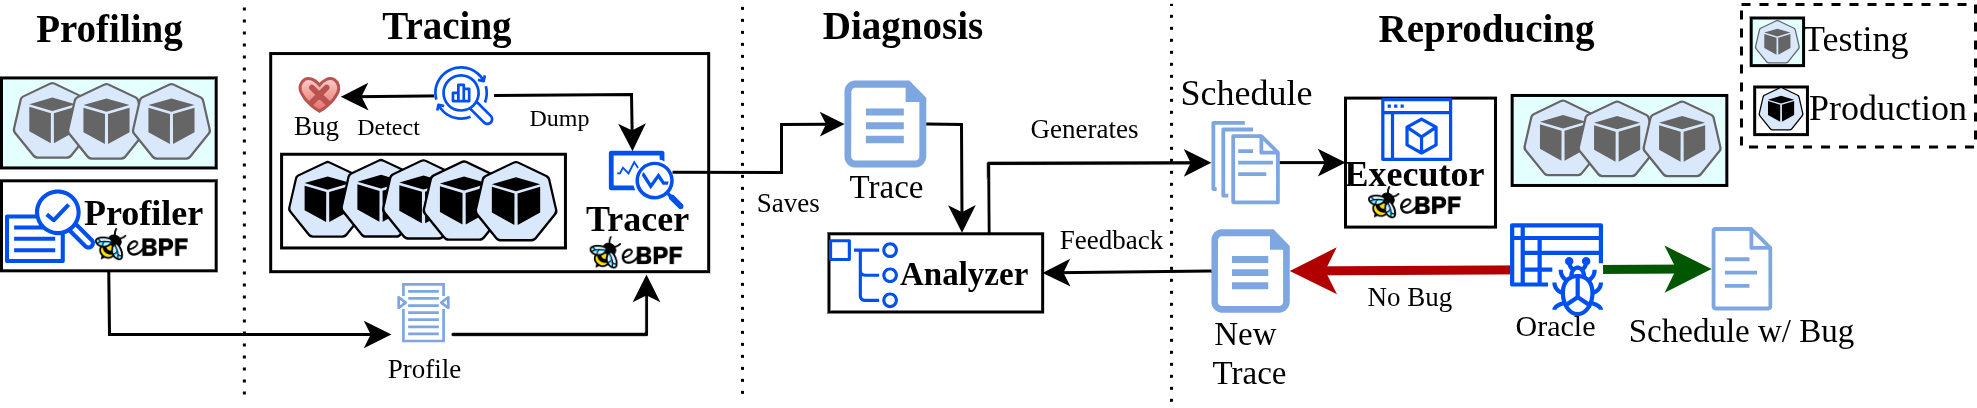
\includegraphics[height=0.16\textheight]{Figures/ROSE-Paper Workflow.png}
	\caption{Workflow of \sys.}
	\label{fig:workflow}
\end{figure*}

\subsection{Target Bugs}
\sa{R2C4,R3C1: New Section }
\label{sec:targetbugs}
In this work, we aim to reproduce \efibshort, these are bugs which are revealed by external faults that occur in the environment.
This is the only condition for \sys to reproduce a bug, the underlying semantics of the bug, recovery, consensus, snapshooting, etc. are not relevant
in this work.
\efibshort that need fine-grained and detailed dataflows are out of our scope, since we do not currently collect information about the inputs and outputs of the system.
If the developer has access to this information, then \sys can reproduce the bug.
\sa{Not sure about adding these lines about data/control}


\subsection{Overview and Workflow}
\label{sec:overview}

To reproduce \efibshort, \sys follows the workflow depicted in Figure~\ref{fig:workflow} which consists of four phases.

\mypara{Profiling phase}. This phase identifies common faults in the system, collects system call frequency, and optionally identifies infrequent functions that might represent important system state changes.

\mypara{Tracing phase.} This phase deploys a production tracer to capture relevant system events.
When a bug occurs, as indicated by the bug oracle, it dumps the trace to disk.

%iii) \emph{diagnosis phase} - analyzes the trace a identify the \emph{fault context}, conditions necessary for a fault for the bug to occur, and produces a fault schedule,
\mypara{Diagnosis phase.} This phase analyzes the trace to identify \emph{fault contexts} that might trigger the bug and generates the corresponding fault schedules.
Fault contexts correspond to sequences of necessary conditions that must be observed before faults are injected.

\mypara{Reproduction phase.} This phase executes the fault schedule and uses the oracle to check whether the bug is reproduced.
If it did not occur, it passes the information collected during the execution to the diagnosis phase, which will use it to gener ate the next fault schedule.
If the bug is found, it repeats the execution multiple times to assess whether this schedule reproduces the bug with a configurable success rate (we used 60\% in our evaluation).
The workflow terminates once a schedule reproduces the bug with the target success rate or if it can not generate more schedules.

%Attempting to reproduce fault-induced bugs in any type of deployed system creates three key challenges: first, we must decide which information we want to gather and what we can gather due to overhead complications. Second, from this collected information, we must find the key aspects of the execution that led to the bug. Third, we must precisely replay the faults that occurred in the deployment.
%\sys addresses these challenges in the following way: it employs low-overhead tracing to deployed systems based on tracing externally observable behavior common to all systems, keeping a batch of the most recent events in the deployment. When a bug occurs, this batch is saved to disk.

%MM: isto depois é um pouco repeteido na discussão, cortei aqui.
%\mm{uniformizar com termos da intro.}
%The profiling and tracing phases address the \emph{information capture} challenge by determining what information to collect from production systems while maintaining low overhead.
%The diagnosis phase addresses the \emph{fault context} challenge by finding the key aspects of execution that led to the bug and the reproduction phase addresses the challenge of \emph{precise fault injection} by accurately replaying the faults in the right context.
%Next, we describe the design of each phase in detail.


%\sys uses this trace to find what faults occurred by looking for unexpected events.
%With a list of faults, we employ an Algorithm that leverages fault specifics and the events that precede them to find the necessary context for the bug to occur. This is accomplished by iteratively creating best-guess schedules, running them, and leveraging the feedback to create a better guess.
%A high-level workflow of \sys is illustrated in Figure~\ref{fig:workflow}. Developers need to provide a system binary, a list of key system files, a way to deploy the system in a controlled environment, a workload, and an oracle to confirm the presence of the bug.


\subsection{Profiling}
\label{sec:profiling}

\sys can reproduce most bugs (15/20 in our evaluation) using only externally observable behavior.
However, for certain bugs, this information is not enough to build a schedule that reproduces the bug with an acceptable rate.
%This is because some bugs only manifest when the system is in specific states, i.e. executing specific application functions.
This is because some bugs only manifest when the system is executing specific application functions.

The goal of this phase is to identify which of these functions might be relevant through a frequency-based heuristic.
Developers provide a list of functions or files that control critical system functionalities (e.g: recovery procedures, leader change mechanisms, snapshotting, etc).
\sys then runs the system with a representative workload in a failure-free testing environment and counts function invocations, separating them into frequent (a configurable value, defaults to 2 calls per second) and infrequent groups.
Frequently called functions are discarded, and the rest are passed as monitoring sites (in addition to the system calls, monitored by default) to the tracing phase.
The intuition is that \efibshort typically involve code paths that rarely execute during normal operation.
This approach maintains our black-box philosophy by working with any system while providing just enough internal state visibility to capture critical execution contexts.
\sa{R1C7,R3C3: While the names of the files are specific information to the system, for \sys they are only addresses/offsets within a binary. Instead of asking developers to give the addresses themselves, which is a general solution, we think that providing the filenames and having \sys collect the addresses is a simpler approach and makes \sys easier to use.}.

Additionally, we also collect information about any faults that might occur since some faults are common even in failure-free executions, as well as the frequency of system calls in the system, to distinguish between common and rare system calls.
This information is latter used to guide the search in the diagnosis phase.

\subsection{Tracing}
\label{sec:tracing}

\mm{num sistema real teríamos que fazer merge de traces de várias máquinas físicas. Qual é a abordeagem para isto?}
\sa{Concatenar os logs e ordernar pelo tempo, abordado.}
In this phase, \sys monitors the target system, keeping a sliding window of recent relevant events (1 million by default), and provides a \texttt{dump} primitive to write the window to disk.
This primitive is externally invoked either manually by an operator or, more typically, by the existing monitoring infrastructure when a deviation from normal behavior is detected.
The tracer runs on each application node.

\subsubsection{Events} We represent the trace as a sequence of events:

\[Trace = \Big( E_i = \{ts,type,I\} \Big)_{i=1...n} \]
where each event $E_i$ is associated with a timestamp $ts$, the $type$ of event, and event specific information $I$.
There are four event types.

%The number of events saved (x) has a default value of 1 million, with this approach, we do not consume extra memory/disk space as a naive save-everything approach would.
%\[Trace = \sum_{n=x}^{y} Event \{id,Context,ts,rt\} \ (4)  \]
%Events in \tracer are represented by their id, which represents the type of event, their context, which details specifics about the event, the timestamp at which they occurred, and their relative time. Context is different for all types of events and gives key information about the event.
%It is by looking at sequences of events and their context that we can find clues about what faults happened, and in what context they occurred. The event with the earliest timestamp will be considered the first one, and the relative time of the others will be calculated accordingly.
\mypara{System Call Failures (SCF).}
The most common event is system call failures (SCF).
Even though SCFs are not uncommon, they provide key insights into the (unsuccessful) interactions between the system and the external environment.
The tracer monitors system calls and when they return an error, we record the process id, the system call id~\cite{syscallids}, the file descriptor(for file-related I/O operations), and the \texttt{errno} return code.
For file-related system calls that use the filename instead of the file descriptors, such as \texttt{open} and \texttt{stat}, we capture the filename.
The filename allows us to have a richer context about the possible problematic event, and the \texttt{errno} allows us to later replay and emulate this event.
\[ SCF_I = \{pid, syscall\_id, fd,filename, errno\}  \]

%These failures often indicate external faults (network issues, disk errors) affecting the system.
%The base context for these events is: the pid, the errno return code, and a filename if the system call is related to I/O or other operations on files (e.g. stat). The pid allows us to identify the node, the ID allows us to identify the system call,

%When a node in a production distributed system has a buggy behavior it is revealed to others through system calls. Many incorrect internal mechanisms can happen, but barring the process crashing, being isolated from the network, or stopping, it is when another node makes contact with it that this incorrect state will reveal itself. The same insight applies to application state changes, when a node has a relevant state change, such as going from follower to leader, it is only at the point at which this change becomes external that it becomes known to the overall system.


\mypara{Application Functions (AF).}\label{userfunc}
The tracer also captures the infrequent function invocations, capturing important information about application state changes.
We record the process id and a function id, a unique integer associated with each function defined during the profiling phase.
\[ AF_I = \{pid, function\_id\}  \]

%Note that to keep tracing as lightweight as possible we do not capture any further information about the function such as function parameters.
%We will further discuss the impact of this in \S\ref{sec:diagnosis}.


\mypara{Network Delays (ND).}\label{networktracing}
Network partitions and failures are a common cause of \efibshort.
Network failures capture a wide-range of general behaviors such as packet loss, link flapping, or latency spikes, among others, while network partitions capture specific failure patterns where the system is split into two or more subsets of nodes: nodes are able to communicate with other nodes within the subset but not with nodes in other subsets (either in one or both directions).

While some network failures can be captured as system call failures (e.g.: a \texttt{connect} failure) others cannot (e.g.: latency spikes).
Temporary network partitions/failures also pose a problem --- while, for instance, a failed \texttt{connect} might indicate the beginning of a network partition, since we do not track successful system calls we are not able to detect when the partition is healed.
We therefore need a more robust method of detecting network issues and their duration.

Since periods of network inactivity may indicate partitions or connectivity issues, we employ a strategy that aims to detect network delays (ND) as a proxy for identifying possible network failures or partitions.
We detect these delays by keeping a map of active connections.
When a node sends a packet, we calculate the delay between this packet and the last time a packet was sent in this connection.
If the delay is longer than configurable value (5 seconds by default), we record a network delay event, containing the source and destination IPs, the duration, and the number of packets sent in the connection up until this moment.
\[ND_I = \{Dest\_IP , Source\_IP , Duration, Packet\_Count\}  \]


\mypara{Process States and Restarts (PS).}
Process crashes and pauses are other common source of \efibshort where the crash/pause of a process triggers a cascading effect in the rest of the system.
We monitor this by keeping track of the process state --- if a process is in the \texttt{waiting} state for more than a configurable time (3 seconds by default), we record this as a possible fault.
We also create an event when a  process crashes.
We record the process id, the state of the process, and for process pauses, the duration of the pause.
%Processes crashes can be detected by the above solution, however, a restart can not. This is because when an application node starts again, it is assigned a new pid, which the tracer is not aware of. We ask developers to provide information about the node when it reboots to the tracer, so the tracer can create the necessary infrastructure to trace this new process. This is a simple write to a file with application node name, and pid.
\[PS_I = \{pid, State, Duration\}  \]
%\mm{como é que a duração é medida se um processo tiver 9 secs em waiting? são 3 eventos de duração 3? ou 1 evento de duração 9? o State é apenas waiting? Ou crashed? O restart é também um state?} \sa{Mais que 3 segundos, corrigido no texto}
%\mm{mas se a falha demoara 9 segundos quantos events ~são gerados? 1 com Duration=12 ou 4 com Duration=3?}\sa{Duration=9}
%MM a consequência disto é que se a pausa continuar e se fizer o dump não vemos esse evento no log. Deveríamos ter uma forma mais sistemática de lidar com isto, por exemplo emitindo eventos pendentes quando se faz dump.

%\mm{comentei a parte do restart acim{mas se a falha demoara 9 segundos quantos events ~são gerados? 1 com Duration=12 ou 4 com Duration=3?}, acho que pode ir para a impl. pois creio que isso poderia ser automatizado sem ter que pedir info extra ao utilizador, podemos disctuir depois}


\mypara{Event Duration.}
For events that happen over a time interval, namely network partitions or process pauses, we record their duration and add a single event to the window.
This minimizes the number of events, but also implies that we have to be careful when handling events that did yet terminate when a \texttt{dump} is requested.
For process pauses, if there are ongoing pauses, we save them to the trace.
For network partitions, we check the delay between the last seen packet and the current timestamp and add it to the trace if it surpasses the configured delay for detecting network partitions.

%The trace is then passed to the \emph{diagnosis Phase} which we discuss next. If deployed on multiple machines, we first concatenate the different traces according to their timestamps.
If the tracer is deployed on multiple nodes, we first merge the traces before passing them to the next phase.
%(\S\ref{sec:diagnosis}) which analyzes the events, iteratively refines the execution context, and outputs fault schedules.


\subsection{Diagnosis}

\begin{figure*}[htbp]
	\centering
	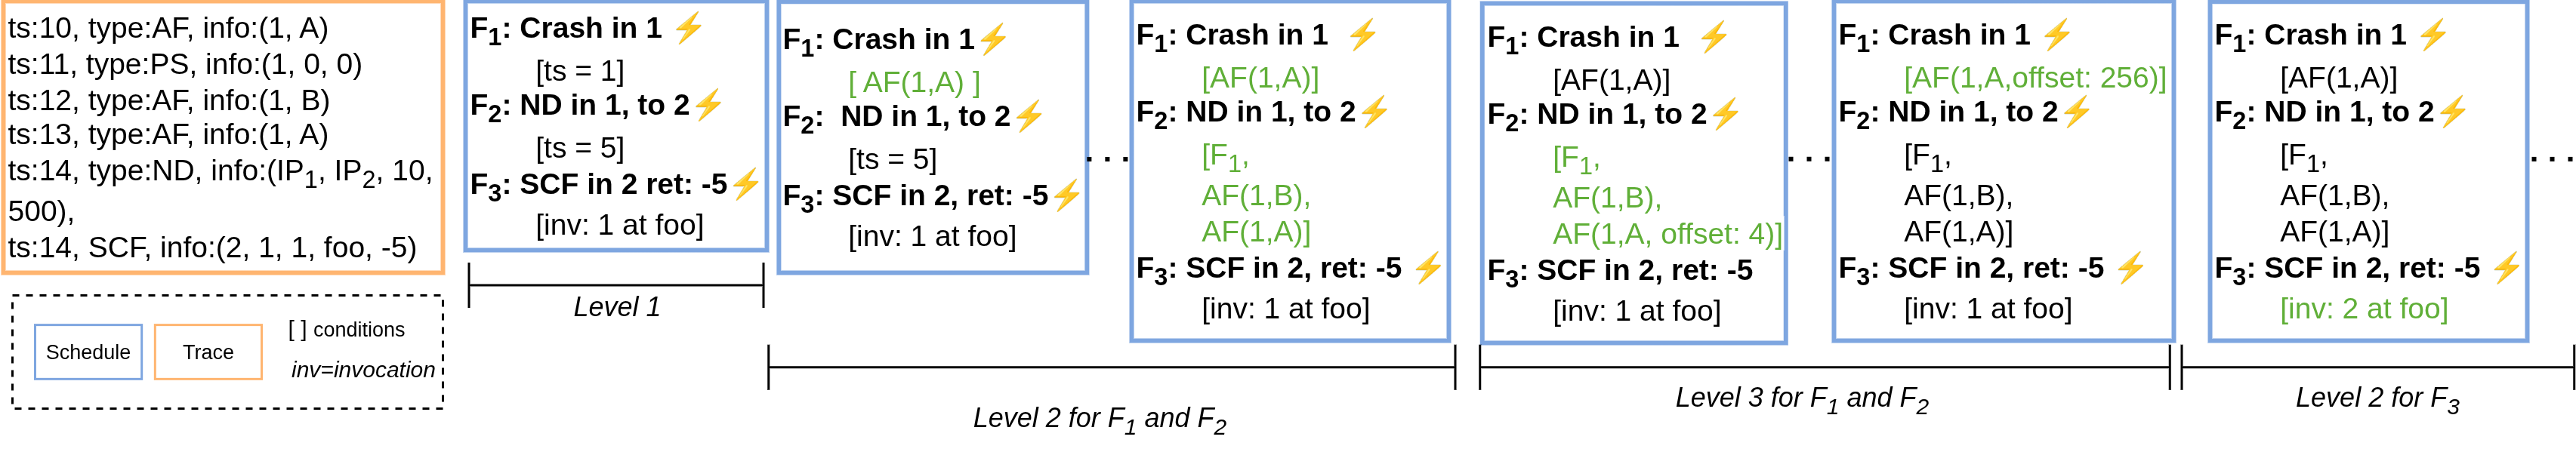
\includegraphics[height=0.135\textheight]{Figures/ROSE-Levels.png}
	\caption{Diagnosis Phase.}
	\label{fig:levels}
\end{figure*}


\label{sec:diagnosis}
The goal of this phase is to identify the necessary \emph{fault context} in which faults should occur, and output a \emph{fault schedule} that reproduces the \efibsingle .
We define \emph{fault context} as the sequence of necessary conditions that must be observed before a fault is injected.
These conditions might include invocation of application-specific functions (AF), particular process states (PS) and network delays (ND), and other system call failures (SCF).
Note that we do not aim to perform root cause analysis and pinpoint the root of the \efibsingle, but instead to quickly create a fault schedule that triggers the bug with a high replay rate.
This creates tension between precision (capturing the right conditions) and relevance (creating a minimal schedule that consistently triggers the bug).

To this end, we employ an iterative algorithm that starts with a basic context (the information of the faults themselves) and iteratively contextualizes each fault, with either the AF events that preceded it, or in the case of SCF, different invocations.
For every iteration, the algorithm outputs a schedule that is passed to the next phase for execution.
If the schedule triggers the bug with a configurable replay rate, we stop, otherwise we refine the schedule based on the execution feedback and try again.
The algorithm builds the fault context in three different levels, as depicted in Figure~\ref{fig:levels}.


\subsubsection{Level 1: Initial Guess.}
\label{sec:levelone}
The algorithm starts by collecting all the faults in the trace.
\sa{R2C1: However, we can not iterate through all the benign faults (faults which do not cause a bug in a system), as this would be an unfeasible task. Thus, we compare a normal execution with the trace obtained from production to discard benign faults.}
\sa{Should I give examples of this here, or in the evaluation?}
Given this set of faults, the challenge is how to select which ones to contextualize first, to create a schedule within an acceptable time.
We prioritize faults based on their potential impact on the system and their expected frequency, with less frequent faults having more priority, as well as faults that are in the trace but have not been observed during the profiling phase.
In detail, we prioritize first PS, then ND and finally SCF, and within each category we follow chronological order.
The rationale is that later faults might be due to earlier faults and hence be a symptom rather than a cause.

The algorithm then traverses the sorted list of faults, creating a fault schedule without context and only including the faults' information (fault order, inputs for system calls).

The key insight is that some bugs do not need a particularly complex application state and can be revealed by simply injecting the faults in the correct order.

As an example, for bug \texttt{ZOOKEEPER-3006} (Table~\ref{tab:bugs}), injecting a SCF when opening the snapshot file was enough to reveal the bug.
For SCF we inject the fault by manipulating the error code.
For PS we crash or pause the process for the relevant time.
For ND we inject the respective fault for the duration observed in the trace.
Despite its simplicity, this level quickly identifies \efibshort with straightforward trigger conditions and can create a schedule with 100\% replay rate for 10/20 bugs (Table~\ref{tab:bugs}).

\subsubsection{Level 2: What happened before?}
\label{sec:leveltwo}
If Level 1 fails, we expand the context by triggering the faults at different application states, considering application-specific functions as illustrated in Figure~\ref{fig:levels}.

\mypara{System calls.}
To contextualize system calls where we have input information (e.g.: the filename), we generate schedules that fail the system call at different invocation counts.
As an example this could be failing the first write to a given file, then in the next schedule the second write, and so on.
For system calls where we do not have inputs, we attempt to fail the system call the number of times it appeared in the profiling trace, with a hard cap of attempts (50 by default).
As an example, bug \texttt{HDFS-15032} (Table~\ref{tab:bugs}) is triggered 100\% of the times by injecting a fault in a specific \texttt{connect} invocation.

\mypara{Process and Network faults.} Since these faults do not have context information other than their timestamp and duration, we use previous invocations of AF as context.
The procedure is depicted in Algorithm~\ref{alg:context} and is based on the insight that faults trigger specific code paths to handle them.

\newcommand{\schedule}{$S$}
\newcommand{\fault}{$F$}
\newcommand{\node}{$N$}
\newcommand{\context}{$L$}
\newcommand{\functions}{$AF$}
\newcommand{\runschedule}[1]{\texttt{runSchedule}(#1)}
\newcommand{\oracle}[1]{\texttt{oracle}(#1)}
\newcommand{\confirmbug}[1]{\texttt{confirmBug}(#1)}
\newcommand{\processtrace}[1]{\texttt{processTrace}(#1)}
\SetKwComment{Comment}{$~\triangleright~$}{}
\DontPrintSemicolon
\SetCommentSty{textsf}
\SetKwComment{Comment}{$~\triangleright~$}{}
\SetKwProg{Fn}{fn}{}{end}
\SetKwProg{Upon}{upon}{}{end}
\SetKwIF{If}{ElseIf}{Else}{if}{then}{elif}{else}{endif}
\SetKw{is}{is}
\newcommand{\Update}{\texttt{UpdateShadowPM}()}
\begin{algorithm}[t]
	\scriptsize
	\caption{Context Creation for Process Faults and Network Faults}\label{alg:context}
	% \linespread{1.10}
	\schedule\Comment{Schedule after Level 1 is Executed}
	\fault\Comment{Fault we are creating the Context for}
	\node\Comment{Node where the fault occured}
	\functions\Comment{Functions called by \node which precede \fault~in production trace}
	\context\Comment{List of unique functions to serve as context for F }

	\SetKwFunction{findContextforFaultfn}{findContextforFault}
	\newcommand{\clr}{cacheline\_reords}
	\newcommand{\getcachelinereords}[1]{\texttt{GetCachelineReorderings}(#1)}
	\newcommand{\apply}[1]{\texttt{ApplyState}(#1)}
	\Fn{\findContextforFaultfn{\schedule,\fault,\node,\functions}}{
		\context $\leftarrow \varnothing$\;
		\For{$f~in$ \functions}{
			\lIf{$f~in$ \context}{
				\Return{\context}
			}
			\schedule[\fault] $\leftarrow$  \schedule[\fault] $+$ $f$\;
			$trace \leftarrow $ \runschedule{\schedule}\;
			$bug \leftarrow $ \oracle{} \;
			\If{$bug$}{
				$replayrate \leftarrow$ \confirmbug{\schedule} \;
				\lIf{$replayrate > 60$}{ \Return{\schedule}}
			}
			$(correctOrder,faultInjected) \leftarrow $ \processtrace{$trace$}\;
			\If{$correctOrder~\&~faultInjected$}{
				\context $\leftarrow$ \context $+ f$ \;
				$continue$
			}
			\schedule[\fault] $\leftarrow$
			\lElse{ \Return{\context} }
		}
	}

	\SetKwFunction{confirmbugfn}{confirmBug}
	\Fn{\confirmbugfn{\schedule}}{
	$bugRuns \leftarrow 0$ \;
	$correctRuns \leftarrow 0$ \;
	\For{$run~in [0:10]$}{
	\Comment{If we can not reach our standard rate we leave}
	\lIf{$correctRuns > 3$}{\Return{$0$}}
	$run(S)$\;
	$bug \leftarrow$ \oracle{}\;
	\lIf{ $bug$}{ $bugRuns+=1$}
	\lElse{ $correctRuns+=1$}
	}
	{ \Return{$(bugRuns/10)*100$} }
	}

	\SetKwFunction{processtracefn}{processTrace}
	\Fn{\processtracefn{$trace$,\fault,\functions$Original$,$SsizeL$}}{
		$AF\_trace \leftarrow $ $get\_AF(trace,F)$\;
		\Comment{Compare behavior in production and caused by schedule}
		$correctOrder \leftarrow $ $AF\_trace[0:sizeL]$ == \functions$Original[0:sizeL]$\;
		$faultInjected \leftarrow$ \fault~$in$ $trace$ \;
		\Return{$(correctOrder,faultInjected)$}

	}
\end{algorithm}


We denote faults with $F$ and functions with $f$.
For a given fault $F$, observed on node $N$, the goal is to create a list of unique functions ($L$) to serve as \emph{fault-context} for $F$.
Given the function $f$, that immediately preceded $F$ on $N$, we execute a schedule $S$, where $F$ occurs after $f$ (line 10).
Next, we check for the bug with the provided oracle; if it is present, we confirm if $S$ has the target replay rate (line 14).
If yes, we return $S$ and finish the process, otherwise we continue.
If we observe $L$+$f$ functions in the testing run in the same order as production but the bug is not triggered, it means our sequence is not precise enough to reproduce the bug.
Thus we add $f$ to $L$ (line 18), and move to the next function (line 19).
If we do not observe $f$ in the run, then $F$ is not injected.
This means that $f$ is not likely part of a specific code path to trigger the bug and thus we move to the next fault (line 20).

To generate a new schedule, we search for the function $f+1$ that immediately precedes $f$.
If $f+1$ is not in $L$, we add it to the schedule and execute, repeating the process (line 10).
If $f+1$ is already in the schedule, it means we are no longer in a unique code path, and we move to the next fault (line 9).
The intuition is that functions that occur once are more likely to indicate relevant application-specific states.
\sa{R1C1: While ignoring the duplicate and continuing is a possible option, it would make the algorithm run significantly longer, since \sys would try to construct a context with all the unique functions detected.}

\mypara{Role-specific State.} In many systems, different nodes can assume different roles such as the primary replica in a primary-backup database deployment.
Thus, when a fault occurs, different nodes might show different behaviors contingent on the assumed role.
To handle these scenarios, we employ an \emph{Amplification} heuristic that replicates the schedule across all nodes to determine whether the triggering context is role-specific.
We do \emph{Amplification} if we did not observe $f$ in the testing run.
If $f$ does not appear in any node, it means the context is not role-specific, and we revert this step.
If $f$ appears on some nodes, we leave the schedule as is.
We do not employ this for network faults, since they have consequences on the entire deployment.

%If the fault context is observed in all nodes then this means it is not role specific. \mm{e depois?} Otherwise, we extend the schedule as discussed above and repeat the amplification step.

\mypara{Fault Order.} To faithfully replay what occurred in production we enforce in testing the fault order that was observed in production as detailed in \S\ref{sec:repr:state}.
%However this causes a problem, for example, in a schedule with Faults $A$ and $B$, with contexts $C_A$ and $C_B$.
%When this schedule is run, there is a possibility that $C_B$ occurs before $C_A$, and therefore, the faults would be injected in the reversed order of what was observed in production.
%We address this by enforcing a order between faults, as detailed in \S\ref{sec:repr:state}.

\mypara{Prunning runs.} During fault contextualization, bugs sometimes manifests below the target replay rate due to either incomplete fault contextualization or imprecise context identification.
To address this variability, when we first detect a bug with fault $F$, we immediately evaluate its replay rate.
If we have already seen it, we save the schedule as a possible candidate, and in the end check the replay rate of all candidates.

As an example, reproducing \texttt{RedisRaft-51} (Table~\ref{tab:bugs}) requires injecting the fault when the leader sends the snapshot to other nodes which is role-specific and hence requires the amplification step.
%thus, this bug requires the right fault schedule with the \emph{Amplification} heuristic.


\subsubsection{Level 3: Function-specific context}
\label{sec:levelthree}
In the previous level, and since we capture only the function invocations without any parameters, the faults are injected at the function return point.
Naturally, this misses the fact that functions can contain multiple execution paths, only some of which might be relevant for triggering and reproducing \efibshort.
This can be the difference between a failed and a successful reproduction.
With this in mind, this level creates more refined schedules that inject faults at specific offsets within the functions that immediately precede each fault.
Rather than testing all offsets in sequence, or at random, we prioritize as follows:
i) call sites to system calls,
ii) call sites to other functions, which can reveal system state changes relevant to the bug, and
iii) the rest of the offsets.

For example, reproducing \texttt{RedisRaft-NEW} requires crashing a node executing a \texttt{write} within a specific function.
This corrupts the snapshot and prevents the node from restarting.

\subsection{Reproduction}
\label{sec:reproducing}

This phase executes the target system with the provided workload in the testing environment and injects the faults specified in the fault schedule.
We assume that the developer can provide a representative workload that is able to exercise the relevant code paths that might trigger the bug.
After each execution, we use the bug oracle to infer whether this schedule triggers the bug or not.
In practice, the oracle can be implemented by parsing logs to look for specific errors, automated tools such as Elle~\cite{elle} that check for invariants over the system state, or health checks performed by the production monitoring system, among others.


If the bug is found, the execution is repeated with the same schedule to confirm whether it is able to reproduce with the target replay rate (60\% by default).
Otherwise, the information collected during the execution is fed back to the diagnosis phase, specifically, the information about injected faults and their contexts (lines 34 and 35 in Algorithm~\ref{alg:context}).

The main component of this phase is an \emph{Executor} which:
i) keeps track of the system state;
ii) evaluates the current system state and determine whether a fault needs to be injected; and
iii) injects the actual fault.

\subsubsection{State Tracking}
\label{sec:repr:state}

Since different nodes are likely to be subject to different faults during a testing run, we start by pre-processing the fault schedule to determine which events apply to which node.
Next, we determine for each node the conditions that should be observed in order to inject a fault.

A condition can be a function call, a system call counter, or a system call counter with specifications about their inputs, e.g. the number of times that \texttt{open} must be called with a specific path.
Finally, to preserve the fault order observed in production, we add as conditions to the fault any previous faults that might appear in the trace.
This prevents premature or out-of-order fault injection and eliminates a source of randomness, contributing to better replay rates.
For example in Figure~\ref{fig:levels}, function $A$ is part of the \emph{fault context} of fault $F_2$, meaning we must observe $A$ after injecting $F_1$ in order to injecting $F_2$.
Otherwise, if we observed $A$ before injecting $F1$, this would cause us to inject $F2$ before $F1$ violating the fault order observed in production.
%Thus, we employ the strategy above to enforce the order we saw in production.


%We also leverage time as a condition, time is not a precise metric of system state, but some faults do not need specific context information. Time also allows us to keep a casual order between faults, which depend on function call counters. If time is present as a condition the other conditions will only be taken into account if time is already set. This allows us to keep a casual order between the faults while also making sure they occur after their chains.


\subsubsection{Fault Injection}
\label{sec:overview:fi}
%When all the conditions are satisfied, the fault is injected exactly at the next event where the fault can be triggered.
%When all but one condition for a fault are satisfied, and we encounter the last one, the fault is executed exactly at that system state.
When we observe the last condition that satisfies the fault context, the fault is immediately injected.
The key concern when injecting faults is ensuring precision, i.e. that faults are injected exactly at the same point in the application state across testing runs.
The low-level mechanisms to inject the faults are tied to eBPF's functionalities and are discussed in more detail in the implementation (\S\ref{sec:implementation}), here we focus only on the high-level design and goals.
To fail system calls, we override the return value with the one described in the fault schedule, and completely skip the logic of the system call.
This emulates a scenario where the system call failed right at the beginning of the invocation.
Since we can not know from the production trace whether the system call completed, we opt not to completely skip their execution and return the error code observed in production.
This decision is based on the fact that skipping a system call is a faulty behavior and by returning an error, we force the system to go into the code paths that handle faults.
For process pauses and crashes, we send a signal from kernel space to the target process which ensures the process is crashed/paused consistently in the same state.
For network faults, we drop packets between the target processes as specified in the schedule to emulate a network delay or a network partition.
